%%%%%%%%%%%%%%%%%%%%%%%%%%%%%%%%%%%%%%%%%%%%%%%%%%%%%%%%%%%%%%%%%%%%%%%%
%                                                                      %
% LaTeX, FIIW thesis template                                          %
% 28/11/2014 v1.2                                                      %
%                                                                      %
%%%%%%%%%%%%%%%%%%%%%%%%%%%%%%%%%%%%%%%%%%%%%%%%%%%%%%%%%%%%%%%%%%%%%%%%
\documentclass[11pt,a4paper]{report}
% Indien je je thesis recto-verso wil afdrukken gebruik je onderstaande opties i.p.v. bovenstaande
%\documentclass[11pt,a4paper,twoside,openright]{report}

\usepackage[a4paper,left=3.5cm, right=2.5cm, top=3.5cm, bottom=3.5cm]{geometry}
\usepackage[dutch]{babel}
\usepackage{graphicx}
\usepackage[latin1]{inputenc}           % om niet ascii karakters rechtstreeks te kunnen inputten
%\usepackage[utf8]{inputenc}            % commentarieer deze regel uit als je utf8 encoded files gebruikt in plaats van latin1
\usepackage{natbib}
\usepackage{listings}             		% voor het weergeven van broncode
\usepackage{verbatim}					% weergeven van code, commando's, ...
\usepackage{hyperref}					% maak PDF van de thesis navigeerbaar
\usepackage{url}						% URL's invoegen in tekst met behulp van \url{http://}
\usepackage[small,bf,hang]{caption}     % om de captions wat te verbeteren
\usepackage[final]{pdfpages}            % gebruikt voor het invoegen van het artikel in pdf-formaat
\usepackage{pslatex}					% andere lettertype's dan de standaard types

\usepackage{sectsty}					% aanpassen van de fonts van sections en chapters
\allsectionsfont{\sffamily}
\chapterfont{\sffamily}

\usepackage{float}                      % De optie H voor de plaatsing van figuren op de plaats waar je ze invoegt. bvb. \begin{figure}[H]
\usepackage[dutch]{varioref}
\usepackage{graphicx}
\usepackage{amsmath}
%\usepackage{longtable}					% tabellen die over meerdere pagina's gespreid worden
%\usepackage[times]{quotchap}           % indien je fancy hoofdstuktitels wil
%\usepackage[none]{hyphenat}
%\usepackage{latexsym}
%\usepackage{amsmath}
%\usepackage{amssymb}

\usepackage{fiiw_gent}
% \usepackage{fiiw_ghent_eng} % For the english version (also change last page at the bottom of this file!

%door onderstaande regels in commentaar te zetten, of op false, kan je pagina's weglaten
%bijvoorbeeld het weglaten van een voorwoord, lijst met symbolen, ...
%%%%%%%%%%%%%%%%%%%%%%%%%%%%%%%%%%%%%%%%%%%%%%%%%%%%%%%%%%%%%%%%%%%%%%%%%%%%%%%%%%%%%%%%
%voorwoord toevoegen?
%\acknowledgementspagetrue
%\acknowledgements{voorwoord}			%.tex file met daarin het voorwoord
%abstract toevoegen?
%\abstractpagetrue
%\abstracts{abstract}					%.tex file met daarin het abstract
%lijst van figuren toevoegen?
%\listoffigurespagetrue
%lijst van tabellen toevoegen?
%\listoftablespagetrue
%lijst van symbolen toevoegen?
%\listofsymbolspagetrue
%\listofsymbols{symbolen}				%.tex file met daarin de lijst van symbolen

%informatie over het eindwerk, de promotor, ...
%%%%%%%%%%%%%%%%%%%%%%%%%%%%%%%%%%%%%%%%%%%%%%%
\opleiding{Industri\"ele ingenieurswetenschappen}
\afdeling{Elektronica-ICT: Elektronica}

\title{Ontwikkeling van een self-driving voertuig}
\subtitle{}
\forenameA{Jorik}
\surnameA{De Bruycker}
\forenameB{Jonas}
\surnameB{Bolle}
\academicyear{2017 - 2018}

\promotorA[Begeleiders]{Leenders Guus\\Crul Stijn\\Naessens Carine\\Van Der Perre Liesbeth}
\promotorB[Coach]{Cox Bert}

\begin{document}
\selectlanguage{dutch}
\preface
\tableofcontents

\chapter{Inleiding}
\section{Probleemstelling}
Voor dit project ontwikkelen we een robot/voertuig dat autonoom zo snel mogelijk een raceparcours kan afleggen, dit parcours bestaat uit een zwarte ondergrond afgebakend door volle witte lijnen en een witte stippellijn in het midden. Het prototypen van ons voertuig voeren we uit met behulp van Arduino met een motor shield, tevens ontwikkelen we een custom board om deze Arduino in een later stadium van ons project te vervangen. We voorzien ons voertuig ook nog van enkele andere functionaliteiten. Zo zullen we een snelheidsmeter voorzien. Ten tweede zorgen we ook voor een RFID-reader waarmee ons voertuig de ID's van tags die verspreid over het parcours liggen te kunnen inlezen. Ten slotte moeten we deze data ook allemaal draadloos kunnen verzenden, hiervoor voorzien we Bluetooth-communicatie van onze custom Arduino naar een Raspberry Pi 3.
\section{Doelstellingen}
\begin{itemize}
	\item Voertuig autonoom laten het parcours afleggen
	\item Custom board ontwerpen om Arduino en motorshield te vervangen
	\item Voorzien van een snelheidsmeter
	\item Voorzien van een RFID-lezer om tags uit te lezen
	\item Bluetooth-communicatie tussen Arduino en Raspberry Pi 3 realiseren
\end{itemize}
\section{Structuur}
In volgend hoofdstuk gaan we per doelstelling een analyse maken van de te realiseren doelstelling. We bespreken daaropvolgend de manier waarop we deze doelstelling probeerden te verwezenlijken, met eventuele tegenslagen. Daarna gaan we dieper in op de werkelijke realisatie en manier van aanpak die we hanteerden.
Ten slotte evalueren we onze oplossing en trekken we een conclusie.
\chapter{Analyse en realisatie}
\section{Aansturing van de motoren}
Voor het aandrijven van ons wagentje maken we gebruik van twee motoren die via een H-brug door onze Arduino aangestuurd worden. Met behulp van twee digitale pinnen bepalen we de richting van elke motor afzonderlijk. De snelheid wordt geregeld twee bijkomende pinnen waarbij we Pulse Width Modulation gebruiken.
\section{Bijsturen aan de hand van sensoren}
\subsection{Analyse}
Zoals we reeds vermeldden is het de bedoeling dat ons voertuig een parcours autonoom kan afleggen dat afgebakend wordt door twee volle witte lijnen op een zwarte ondergrond met een witte stippelijn tussen beide. Om dergelijk parcours te kunnen navigeren zullen we onderscheid moeten kunnen maken tussen de witte en zwarte ondergrond, hiervoor hebben we dus sensoren nodig die dit mogelijk maken. Voor dergelijke toepassing kiezen we voor infrarood-sensoren. We zullen hiervoor gebruik maken van de TCRT-5000-sensor, zoals u ziet in figuur~\vref{fig:tcrt5000}. 

\begin{figure}[H]
	\centering
	\includegraphics[height=5cm]{tcrt5000.png}
	\caption{TCRT5000 infrarood sensor\label{fig:tcrt5000}}
\end{figure}

\subsection{Realisatie}
\subsubsection*{Sensor-cel}
De TCRT5000 bestaat uit 2 belangrijke onderdelen: ten eerste hebben we een IR-led , deze led verbinden we met een voorschakelweerstand van $330\,\mathrm{\Omega}$. Ten tweede heeft de TCRT5000 een transistor die zich in essentie als IR-gevoelige weerstand gedraagt, samen met een serieweerstand van $68\,\mathrm{k\Omega}$ vormt dit een spanningsdeler. De IR-led zal infrarood uitstralen naar het oppervlak, naargelang de ondergrond wordt dit al dan niet gereflecteerd. Bij een witte ondergrond zal de reflectie groot zijn en de weerstand tussen collector en emittor bijgevolg zeer klein zijn, omgekeerd hebben we bij een zwarte ondergrond een grote weerstand. We kunnen dus naar gelang de uitgangsspaning zoals u ziet in figuur~\vref{fig:tcrt5000cel} naar een analoge pin een waarde inlezen waaruit we kunnen afleiden of de sensor zich boven een witte of een zwarte ondergrond bevindt. Bij een witte ondergrond zal deze waarde ongeveer $30$ tot $50$ bedragen terwijl een zwarte ondergrond een waarde tussen $\approx 600$ een $800$ resulteert.

\begin{figure}[H]
	\centering
	\includegraphics[height=5cm]{tcrt5000cel.png}
	\caption{Sensor-cel met TCRT 5000\label{fig:tcrt5000cel}}
\end{figure}

\subsubsection*{Multiplexing van sensor-cellen}
Aangezien we slechts over een beperkt aantal analoge ingangen beschikken zullen we de verschillende sensoren moeten multiplexen, hiervoor maken we gebruik van een CD4051BE-multiplexer in figuur~\vref{fig:cd4051be}, de pinout van deze IC vindt u in figuur~\vref{fig:cd4051be_pinout}. We gebruiken deze multiplexer om acht sensoren in te kunnen lezen op \'e\'en analoge pin, hiervoor gebruiken we drie digitale pinnen die de bit selects van de multiplexer aansturen.

\begin{figure}[H]
	\centering
	\begin{minipage}[b]{0.4\textwidth}
		\includegraphics[height=5cm]{cd4051be.png}
		\caption{CD4051BE multiplexer}
		\label{fig:cd4051be}
	\end{minipage}
	\hfill
	\begin{minipage}[b]{0.4\textwidth}
		\includegraphics[height=5cm]{cd4051be_pinout.png}
		\caption{CD4051BE multiplexer pinout}
		\label{fig:cd4051be_pinout}
	\end{minipage}
\end{figure}

\subsubsection*{Sensor-arrays}
Om de positie van ons voertuig te detecteren ten opzichte van een witte zijlijn maakten we twee sensor-arrays van elk vier sensoren die via een multiplexer op een aparte printplaat ingelezen worden in \'e\'en analoge pin. De opstelling van deze sensoren ziet u in figuur~\vref{fig:sensorarray}.

\begin{figure}[H]
	\centering
	%\includegraphics[height=5cm]{sensorarray.png}
	\caption{Sensorarrays en multiplexer\label{fig:sensorarray}}
\end{figure}

Om de processortijd voor het inlezen te minimaliseren lezen we de verschillende sensoren via de multiplexer in aan de hand van Gray-code. De volgorde van inlezen wordt verduidelijkt in table~\vref{table:graycode}.

\begin{table}[H]
	\centering
	\begin{tabular}{|l|l|l|l|l|l|}
		\hline
		\# & Bit Select 2 & Bit Select 1 & Bit Select 0 & MUX-pin & Sensor      \\ \hline
		0  & 0            & 0            & 0            & 13      & Vooraan 2   \\ \hline
		1  & 0            & 0            & 1            & 14      & Vooraan 3   \\ \hline
		3  & 0            & 1            & 1            & 12      & Vooraan 1   \\ \hline
		2  & 0            & 1            & 0            & 15      & Vooraan 4   \\ \hline
		6  & 1            & 1            & 0            & 2       & Achteraan 3 \\ \hline
		7  & 1            & 1            & 1            & 7       & Achteraan 2 \\ \hline
		5  & 1            & 0            & 1            & 5       & Achteraan 1 \\ \hline
		4  & 1            & 0            & 0            & 7       & Achteraan 1 \\ \hline
	\end{tabular}
	\caption{Inlezen van sensoren aan de hand van Grey-code}
	\label{table:graycode}
\end{table}

\subsubsection*{Sturen aan de hand van PID-regeling}
Nu we aan de hand van onze sensoren onze positie kunnen bepalen ten opzichte van de zijlijn moeten we ons voertuig correct laten bijsturen, hiervoor passen we PID-regeling toe. PID-regeling gebeurt aan de hand van een foutwaarde die afleiden uit onze sensorwaarden, we kennen dus aan elke sensor een gewicht toe die een maat geeft voor de afwijking tenopzichte van de witte lijn. Deze gewichten vindt u in tabel~\vref{table:sensorgewicht}.

\begin{table}[H]
	\centering
	\begin{tabular}{lllll}
		\hline
		\multicolumn{1}{|l|}{}           & \multicolumn{1}{l|}{Vooraan 1}   & \multicolumn{1}{l|}{Vooraan 2}   & \multicolumn{1}{l|}{Vooraan 3}   & \multicolumn{1}{l|}{Vooraan 4}   \\ \hline
		\multicolumn{1}{|l|}{Foutwaarde} & \multicolumn{1}{l|}{-3}          & \multicolumn{1}{l|}{-1}          & \multicolumn{1}{l|}{1}           & \multicolumn{1}{l|}{3}           \\ \hline
		&                                  &                                  &                                  &                                  \\ \hline
		\multicolumn{1}{|l|}{}           & \multicolumn{1}{l|}{Achteraan 1} & \multicolumn{1}{l|}{Achteraan 2} & \multicolumn{1}{l|}{Achteraan 3} & \multicolumn{1}{l|}{Achteraan 4} \\ \hline
		\multicolumn{1}{|l|}{Foutwaarde} & \multicolumn{1}{l|}{3}           & \multicolumn{1}{l|}{1}           & \multicolumn{1}{l|}{-1}          & \multicolumn{1}{l|}{-3}           \\ \hline
	\end{tabular}
	\caption{Gewichten van sensoren}
	\label{table:sensorgewicht}
\end{table}

De foutwaarde van de voorste sensoren wordt nu berekent met volgende formule:
\begin{gather*}
E_{vooraan} = \frac{\sum\limits_{i=1}^{4}S_{vooraan,i}\cdot G_{vooraan,i}}{\sum\limits_{i=1}^{4}S_{vooraan,i}}
\end{gather*}
Analoog wordt de foutwaarde voor de achterse sensoren gegeven door:
\begin{gather*}
E_{achteraan} = \frac{\sum\limits_{i=1}^{4}S_{achteraan,i}\cdot G_{achteraan,i}}{\sum\limits_{i=1}^{4}S_{achteraan,i}}
\end{gather*}
Hierien is $S_i$ gelijk aan $1$ indien sensor $i$ een witte ondergrond ziet en $0$ wanneer de ondergrond zwart is. $G_i$ is het gewicht van de sensor in kwestie.\\
De totale foutwaarde wordt dan bepaald door beide foutwaarden op te tellen. Deze foutwaarde zal negatief zijn wanneer het wagentje teveel naar rechts afwijkt ten opzichte van de zijlijn, omgekeerd is deze fout positef als het wagentje te veel naar links rijdt. Als het wagentje perfect rechtdoor rijdt zullen de sensorwaardes elkaar compenseren zodat de foutwaarde $0$ wordt. In het geval dat de voorste sensorarray van de baan afwijkt stappen we af van de PID-regeling en laten we het wagentje aan de hand van de laatst bepaalde foutwaarde terug sturen naar de lijn, wanneer de voorste sensorarray zich opnieuw boven de lijn bevindt hervatten we de PID-regeling.
\section{Custom board}
\subsection{Analyse}
\subsection{Realisatie}

\section{Snelheidsmeting}
\subsection{Analyse}
Voor het meten van de snelheid zullen we moeten bepalen hoeveel rotaties de wielen maken gedurende een bepaalde periode. Uit dit aantal rotaties kunnen we vervolgens de afgelegde weg en dus ook de snelheid berekenen. We hebben dus een manier nodig om te detecteren wanneer en hoeveel keer het wiel een rotatie maakt, daarvoor kozen we voor het gebruik van een Hall-sensor die het passeren van magneten gemonteerd in de wielas detecteert. De gebruikte Hall-sensor is een SS41 digitale Hall-sensor van Honeywell die gevoed wordt op $5\,\mathrm{V}$.	
\subsection{Realisatie}
In figuur ~\vref{fig:wielmagneten} ziet u de magneten die binnen in de wielas gemonteerd werden. Deze twee magneten zorgen er voor dat de output van de SS41 omschakelt van hoog ($5\,\mathrm{V}$) naar laag ($0\,\mathrm{V}$) bij het naderen van de sensor en vice versa bij het voorbijgaan. In figuur~\vref{fig:hallsensor} ziet u hoe de Hall-sensor bij het wiel gemonteerd is. Binnen een tijdsinterval $\Delta t$ tellen we het aantal keer $C$ dat deze omschakeling optreedt. Het aantal rotaties in dit interval is dan een vierde (sensor schakelt 2 keer om per magneet) van het aantal keer dat de sensoroutput omschakelde. Wetende dat de diamater $D$ van het wiel $7\,\mathrm{cm}$ bedraagt kunnen we de snelheid $v$ als volgt berekenen:

\begin{gather*}
v=\frac{\Delta x}{\Delta t} = \frac{\frac{C}{2\cdot 2}\cdot\pi\cdot D}{\Delta t}
\end{gather*}

\begin{figure}[H]
	\centering
	\begin{minipage}[b]{0.4\textwidth}
		\centering
		%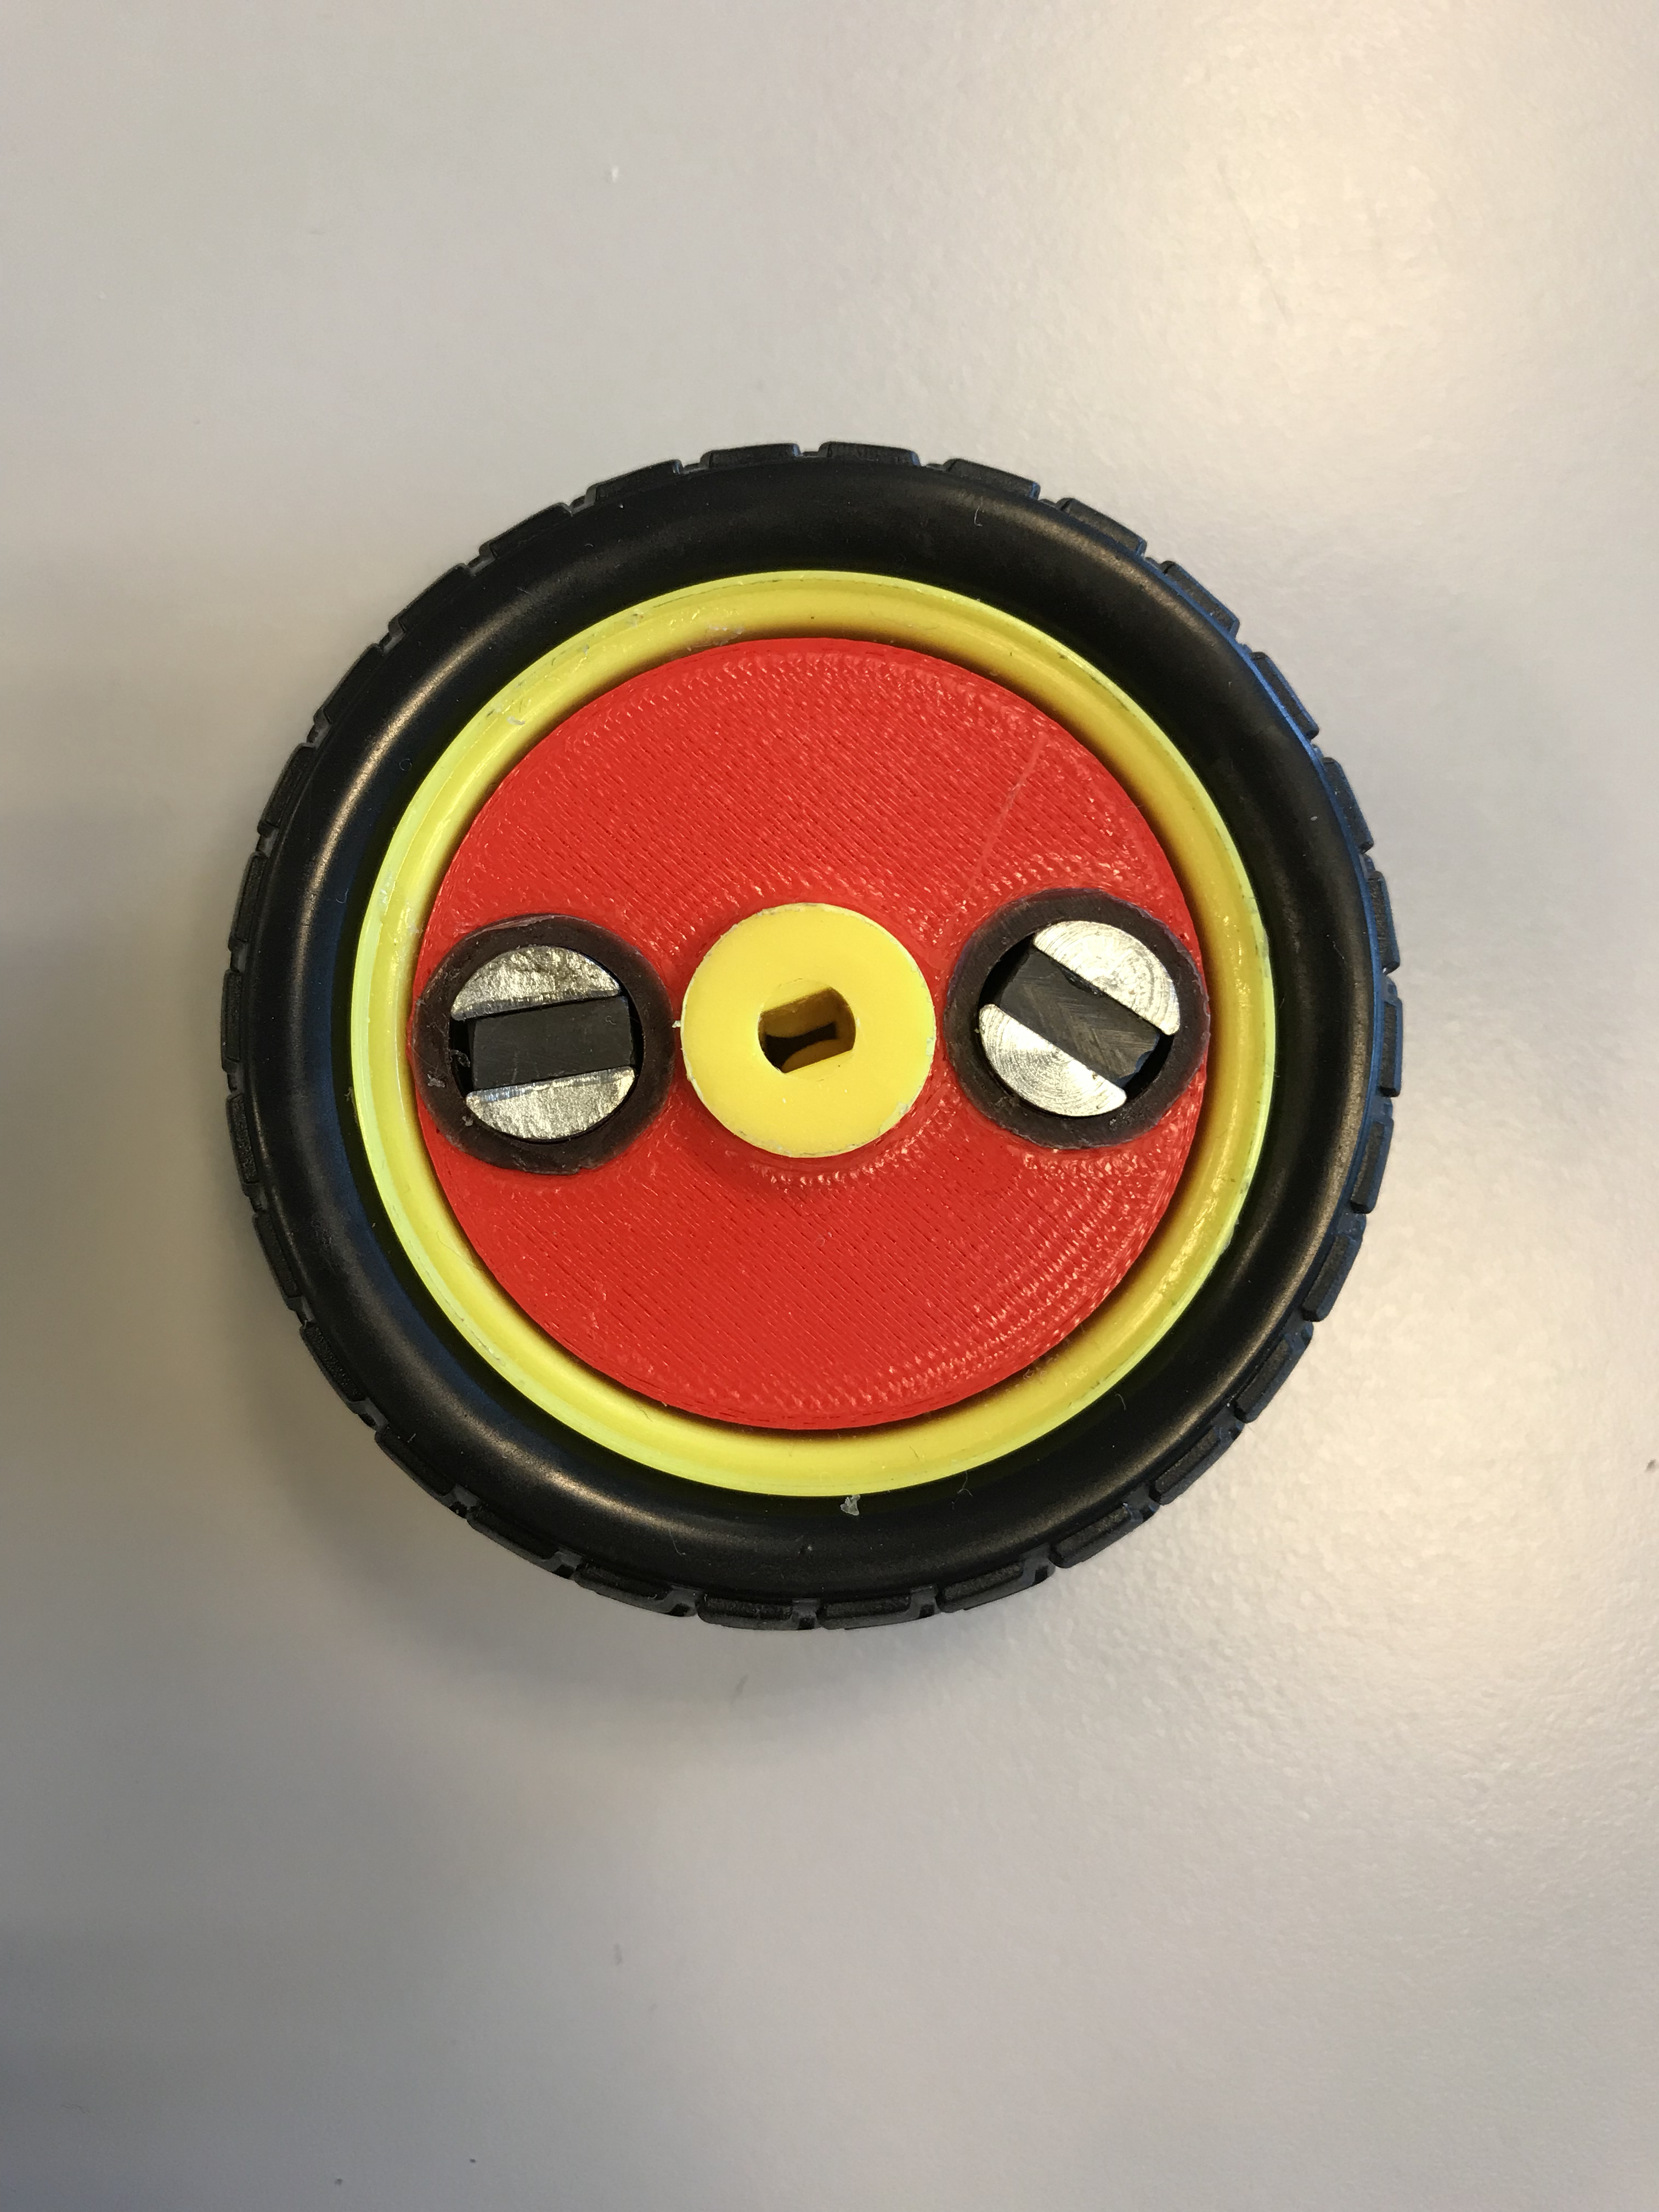
\includegraphics[height=5cm]{wielmagneten.png}
		\caption{Magneten gemonteerd in wielas\label{fig:wielmagneten}}
	\end{minipage}
	\hfill
	\begin{minipage}[b]{0.4\textwidth}
		\centering
		%\includegraphics[height=5cm]{hallsensor.png}
		\caption{Hall-sensor gemonteerd naast wiel\label{fig:hallsensor}}
	\end{minipage}
\end{figure}


\section{RFID-reader}
\subsection{Analyse}
\subsection{Realisatie}
\section{Bluetooth-communicatie}
\subsection{Analyse}
\subsection{Realisatie}
\chapter{Evaluatie}
\chapter{Conclusie}


\includepdf{back_fiiw_gent.pdf}
\end{document}
